\documentclass[12pt,a4paper]{amsart}
% ukazi za delo s slovenscino -- izberi kodiranje, ki ti ustreza
\usepackage[slovene]{babel}
%\usepackage[cp1250]{inputenc}
\usepackage[T1]{fontenc}
\usepackage[utf8]{inputenc}
\usepackage{amsmath,amssymb,amsfonts}
\usepackage{url}
\usepackage{graphicx}
%\usepackage[demo]{graphicx}
%\usepackage[normalem]{ulem}
\usepackage[dvipsnames,usenames]{color}
\usepackage{hyperref}
\hypersetup{
     colorlinks   = true,
     citecolor    = gray
}

\graphicspath{ {./slike/} }
% ne spreminjaj podatkov, ki vplivajo na obliko strani
\textwidth 15cm
\textheight 24cm
\oddsidemargin.5cm
\evensidemargin.5cm
\topmargin-5mm
\addtolength{\footskip}{10pt}
\pagestyle{plain}
\overfullrule=15pt % oznaci predlogo vrstico


% ukazi za matematicna okolja
\theoremstyle{definition} % tekst napisan pokoncno
\newtheorem{definicija}{Definicija}[section]
\newtheorem{primer}[definicija]{Primer}
\newtheorem{opomba}[definicija]{Opomba}

\renewcommand\endprimer{\hfill$\diamondsuit$}


\theoremstyle{plain} % tekst napisan posevno
\newtheorem{lema}[definicija]{Lema}
\newtheorem{izrek}[definicija]{Izrek}
\newtheorem{trditev}[definicija]{Trditev}
\newtheorem{posledica}[definicija]{Posledica}


% za stevilske mnozice uporabi naslednje simbole
\newcommand{\R}{\mathbb R}
\newcommand{\N}{\mathbb N}
\newcommand{\Z}{\mathbb Z}
\newcommand{\C}{\mathbb C}
\newcommand{\Q}{\mathbb Q}

% ukaz za slovarsko geslo
\newlength{\odstavek}
\setlength{\odstavek}{\parindent}
\newcommand{\geslo}[2]{\noindent\textbf{#1}\hspace*{3mm}\hangindent=\parindent\hangafter=1 #2}

% naslednje ukaze ustrezno popravi
\newcommand{\program}{Finančna matematika} % ime studijskega programa: Matematika/Finan"cna matematika
\newcommand{\imeavtorja}{Tina Bertok\\ Neža Habjan \\ Gašper Letnar} % ime avtorja
\newcommand{\imementorja}{prof. dr. Riste Škrekovski} % akademski naziv in ime mentorja
\newcommand{\naslovdela}{Genetski algoritem na problemu potujočega trgovca}
\newcommand{\letnica}{2018} %letnica 




\begin{document}

% od tod do povzetka ne spreminjaj nicesar
\thispagestyle{empty}
\noindent{\large
UNIVERZA V LJUBLJANI\\[1mm]
FAKULTETA ZA MATEMATIKO IN FIZIKO\\[5mm]
\program\ -- 1.~stopnja}
\vfill

\begin{center}{\large
\imeavtorja\\[2mm]
{\bf \naslovdela}\\[10mm]
Projekt v povezavi z OR\\[1cm]}

\end{center}
\vfill

\noindent{\large
Ljubljana, \letnica}
\pagebreak

\thispagestyle{empty}
\hypersetup{linkcolor = black}
\tableofcontents
\pagebreak

\section{Navodilo}

Implement the genetic algorithm metaheuristic for TSP. Present the chromosomes as ordered
lists i.e. as paths. Apply different variations for the crossover operations, such as order crossover
(OX), paritally mapped crossover (PMX), cycle crossover (CX), etc. Experiment with different
sizes of the population. You can generate some of the testing graphs yourself, and you can find
some of them on the Internet.

\newpage
\section{Uvod}

Naša naloga je, da implementiramo genetski algoritem na problemu potujočega trgovca. Pri tem bomo uporabljali različna križanja, spreminjali velikosti populacije in verjetnosti za mutacijo. Primerjali bomo rezultate pri različnih pogojih. Naš algoritem bomo testirali na podatkih, ki jih bomo generirali sami in na podatkih najdenih na internetu. 
\\
\\
\textit{Genetski algoritem} je metahevristika, navdihnjena s strani procesov naravne selekcije in spada v razred razvojnih
algoritmov. Uporablja se za generiranje kvalitetnih rešitev v optimizaciji, ki temeljijo na operatorjih kot so mutacija, križanje
in selekcija.  
\\
V genetskem algoritmu se uporabi množica kandidatov za rešitev, ki jih nato razvijamo do čim boljše rešitve. Vsak kandidat
ima določene lastnosti, katere lahko spremenimo oziroma lahko mutirajo. Evolucija rešitev se ponavadi začne na naključni izbiri kandidatov, katere potem s pomočjo iteracije razvijamo. Na vsakem iterativnem koraku se potem oceni primernost novih kandidatov za optimizacijski problem. Najboljše kandidate potem uporabimo za naslednji korak iteracije. Algoritem se zaključi, ko je izpolnjen zaustavitveni kriterij. Ena možnost je, da algoritem ustavimo po tem, ko preteče določeno število generacij.
\\
\\
\textit{Problem trgovskega potnika} oz. \textit{traveling salesman problem (TSP)} je NP-težek problem v kombinatorični optimizaciji, pomemben pri operacijskih raziskavah, matematični optimizaciji in teoretičnemu računalništvu. Trgovski potnik mora obiskati določeno množico mest tako, da bo pri tem prehodil čim krajšo pot in se vrniti v izhodišče.
\\
\\
Pri programiranju in pisanju algoritma smo se odločili za programski jezik Python, saj imamo v njem največ znanja. Pri projektu pa smo spoznali še knjižnico \textit{matplotlib} za delo z grafi. 
\\

\newpage
\section{Opis dela}


Že dobro poznan problem potujočega , smo se odločili predstaviti z grafom v obliki $n \times n$ matrike cen povezav. Graf smo generirali tako, da smo elemente matrike, ki predstavljajo celoštevilske cene povezav, izbrali naključno. To je prikazano v spodnji funkciji \textit{utezi(n, maxCena)}.

\begin{figure*}[ht]
\centering
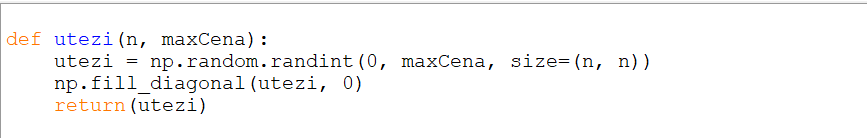
\includegraphics[width=1\textwidth]{utezi}
\end{figure*}

Nato je bilo potrebno definirati \textit{ciljno funkcijo} oz. \textit{fitness function}, s pomočjo katere bomo ocenjevali primernost rešitev. V našem primeru je vrednost te funkcije za neko pot kar dolžina te poti.

\begin{figure*}[ht]
\centering
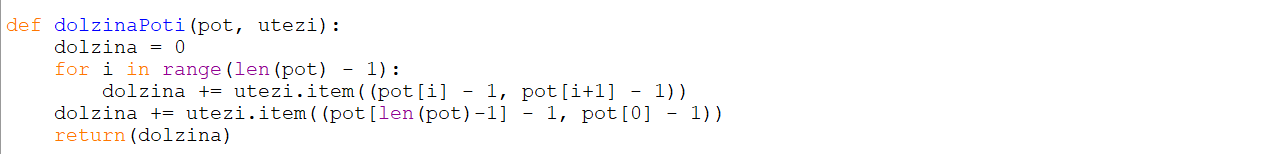
\includegraphics[width=1\textwidth]{dolzinapoti}
\end{figure*}
Naključno smo ustvarili začetno populacijo izbrane velikosti. Vsak element populacije ali \textit{kromosom} predstavlja neko pot, ki obišče vsa vozlišča grafa. 
\\

\begin{figure*}[ht]
\centering
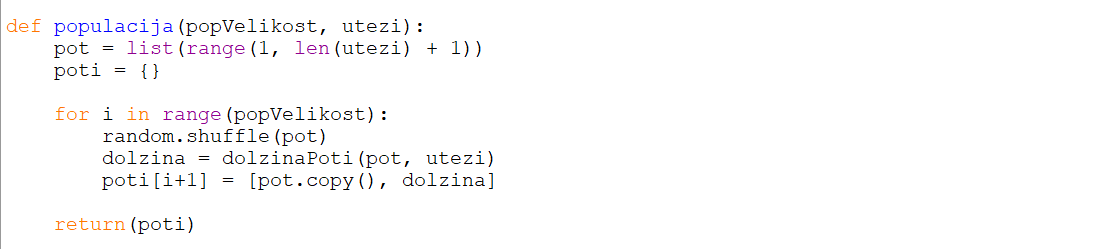
\includegraphics[width=1\textwidth]{populacija}
\end{figure*}
V nadaljevanju izberemo starše, katerih gene bomo uporabili za nastanek naslednje generacije - določimo paritveni bazen. Tega se bomo lotili postopoma in sicer izbiramo po 2 starša za 2 otroka. Za selekcijo imamo dve možnosti, in sicer selekcijo s turnirjem ter proporcionalno selekcijo. Odločili smo se za turnirsko. Vsakega starša bomo izbrali tako, da bomo iz trenutne populacije naključno izbrali  $k$ kromosomov oz. poti. Naša funkcija oz. \textit{selekcija} nam bo vrnila zmagovalca izmed teh  $k$ poti oziroma pot z najkrajšo dolžino. Torej bomo za $n$ staršev v bazenu imeli $n$ turnirjev.

\begin{figure*}[ht]
\centering
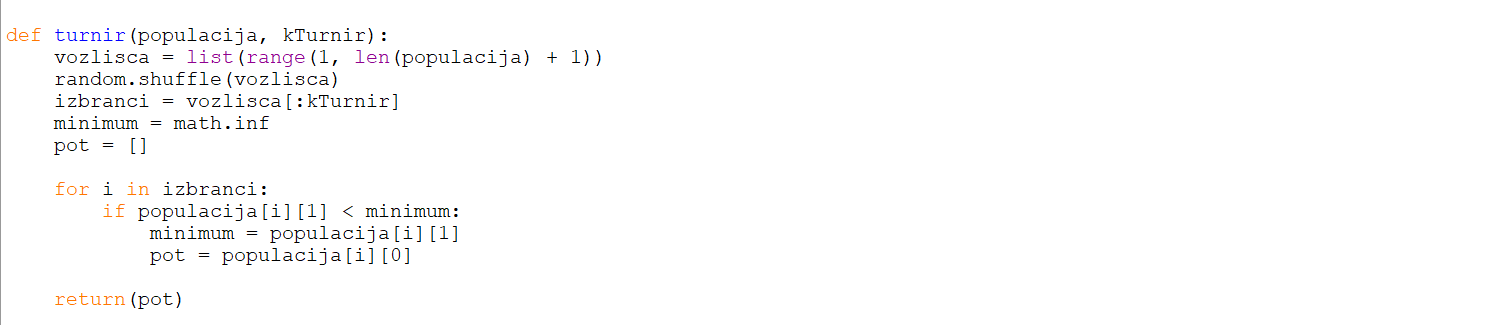
\includegraphics[width=1\textwidth]{turnir}
\end{figure*}

\pagebreak

Za ustvarjanje otrok bomo uporabili različna križanja oz. \textit{crossoverje} staršev (poti) iz paritvenega bazena. Pri tem smo uporabili različne variacije križanj: 
\\
\subsection{Urejeno križanje ali ordered crossover}
\
\\
\\
V urejenem križanju ali OX vsak starš predstavlja neko zaporedje vseh vozlišč. Na začetku oba starša razdelimo na tri podzaporedja, kjer 1. podzaporedje predstavlja vozlišča od prvega do vključno tistega na a-tem mestu, 2. podzaporedje poteka od vozlišča na a-tem do vključno vozlišča na b-tem mestu, 3. podzaporedje pa predstavlja preostanek osnovnega zaporedja. Prvi potomec ima kopirano 2. podzaporedje prvega starša na enaki poziciji. Nato od b+1 mesta naprej nadaljujemo z vozlišči drugega starša, ki jih dopolnjujemo (v primeru da je to vozlišče že vsebovano v zaporedju otroka, ga preskočimo) najprej iz 3. podzaporedja, nato 1. podzaporedja in nazadnje še iz 2. podzaporedja. Ko se zaporedje konča, skočimo na začetek in postopek nadaljujemo vse do začetka a-tega mesta. 
Na enak način tvorimo drugega otroka, le da vlogi staršev zamenjamo.

\begin{figure*}[ht]
\centering
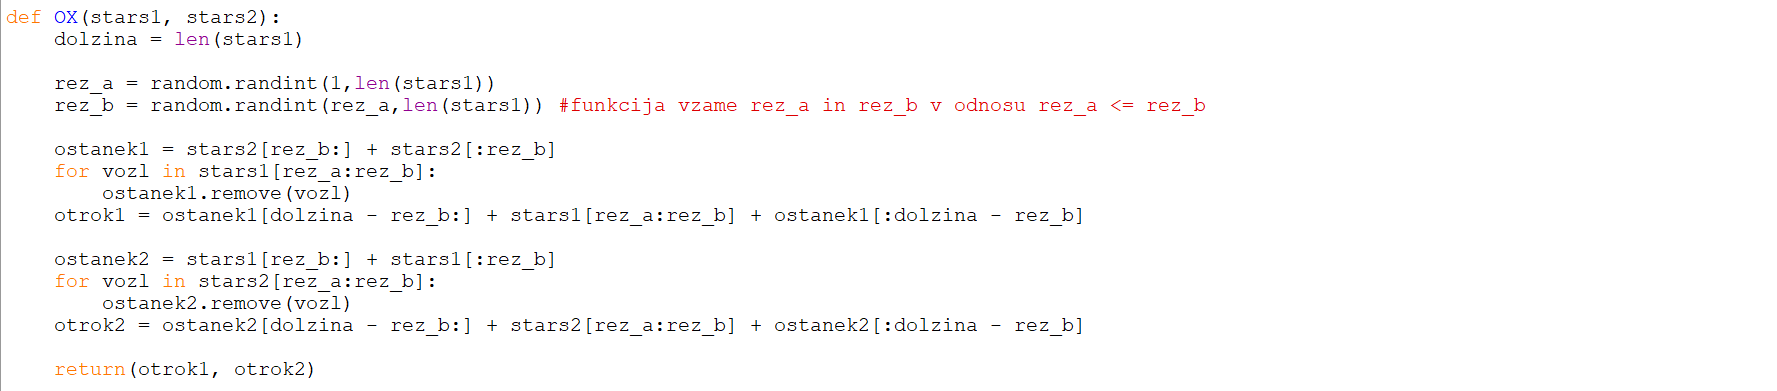
\includegraphics[width=1\textwidth]{OX}
\end{figure*}

\subsection{Delno mapirano križanje ali partially mapped crossover}
\
\\
\\
Drugi način križanja je delno mapirano križanje ali PMX, v katerem starša spet razdelimo na tri podzaporedja. Prvemu otroku prav tako kot v OX, prepišemo vrednosti prvega starša med obema rezoma, se pravi 2. podzaporedje. Nato vsako vozlišče(vsaka vrednost i) iz 2. podzaporedja drugega starša, ki še ni vsebovano v zaporedju otroka, dobi svoj istoležeči par v prvem staršu. Če je ta par že vsebovan v 2. podzaporedju drugega starša, temu vozlišču ponovno poiščemo par iz prvega starša in to počnemo dokler dobljeni istoležeči par v drugem staršu ne leži izven 2. podzaporedja.  Takrat na njegovo mesto (v drugem staršu) zapišemo vrednost i. Na koncu postopka vsa prazna mesta v otroku zapolnimo z istoležečimi vozlišči iz drugega starša. 



\subsection{Ciklično križanje ali cycle crossover}
\
\\
\\
Zadnji način križanja, ki smo ga uporabili je ciklično križanje ali CX. Tu naša funkcija sprejme dva starša, iz katerih naredi slovar. Pri tem prvi starš predstavlja ključ, drugi pa vrednost. Najprej poiščemo vse ciklje med staršema in jih shranimo v množico A. Prvega otroka tvorimo tako, da mu po vrsti dodamo vsak sodi cikel iz prvega stašra in vsak lihi cikel iz drugega starša. Pri drugem otroku ravnamo ravno obratno.  


Tako bomo dobili otroke, ki so neke nove poti ustvarjene iz dveh staršev. Da pa ohranjamo diverziteto v populaciji, bodo nekatere poti mutirane in sicer s \textit{SWAP mutacijo} (zamenjali bomo dve vozlišči v poti). Vsako vozlišče poti z neko verjetnostjo mutiramo, torej zamenjamo položaj mutiranega vozlišča z nekim naključnim vozliščem te poti. 


\newpage
\section{Zaključek}


\begin{thebibliography}{99}


\bibitem{wiki}
\emph{Genetic algorithm}, v: Wikipedia: The Free Encyclopedia, [ogled 13.~12.~201], dostopno na \url{https://en.wikipedia.org/wiki/Genetic_algorithm}.

\bibitem{splet}
N.~Kumar, Karambir in R.~Kumar, \emph{A Comarative Analysis of PMX, CX and OX Crossover operators for solving Travelling Salesman Problem}, [ogled 13.~12.~2018], dostopno na \url{http://www.mnkjournals.com/ijlrst_files/Download/Vol%201%20Issue%202/303-%20Naveen.pdf}.

\end{thebibliography}






\end{document}